% Chapter 02.7: কম্পিউটার নেটওয়ার্কিং: উদ্দেশ্য ও প্রকারভেদ
\section{কম্পিউটার নেটওয়ার্কিং: উদ্দেশ্য ও প্রকারভেদ}

\begin{learningbox}
এই টপিক শেষে শিক্ষার্থী পারবে:
\begin{itemize}
\item কম্পিউটার নেটওয়ার্ক ও networking কী তা ব্যাখ্যা করতে।
\item কম্পিউটার নেটওয়ার্কের উদ্দেশ্য ও প্রয়োজনীয়তা বুঝতে।
\item Resource sharing, data sharing, communication ও centralized management ব্যাখ্যা করতে।
\item PAN, LAN, MAN ও WAN-এর ধারণা, ব্যবহার ও পার্থক্য লিখতে।
\item Client-server network ও peer-to-peer network-এর পার্থক্য বুঝতে।
\item Internet, Intranet ও Extranet-এর basic concept ব্যাখ্যা করতে।
\item বাস্তব scenario দেখে network type শনাক্ত করতে।
\item বোর্ড ও ভর্তি পরীক্ষার জন্য network-based answer লিখতে।
\end{itemize}
\end{learningbox}

\subsection{বাস্তব জীবনের শুরু}

একটি কলেজের computer lab কল্পনা করো। Lab-এর সব computer একটি switch-এর সাথে যুক্ত। শিক্ষক একটি computer থেকে printer share করে দিয়েছেন। শিক্ষার্থীরা একই network থেকে file access করতে পারে, internet ব্যবহার করতে পারে এবং server থেকে class material download করতে পারে।

এখানে computer-গুলো একে অপরের সাথে যুক্ত হয়ে data, printer, internet ও file share করছে। এই ধরনের connected system-ই computer network-এর বাস্তব উদাহরণ।

\begin{keypointbox}{মূল ধারণা}
Computer network বুঝতে ৫টি প্রশ্ন মনে রাখো:
\begin{itemize}
\item কোন কোন device যুক্ত আছে?
\item কী share করা হচ্ছে?
\item connection wired নাকি wireless?
\item network কত বড় area cover করছে?
\item network control centralized নাকি distributed?
\end{itemize}
\end{keypointbox}

\subsection{কম্পিউটার নেটওয়ার্ক}

\begin{definitionbox}{কম্পিউটার নেটওয়ার্ক}
দুই বা ততোধিক computer, device বা node-কে communication medium ও protocol-এর মাধ্যমে যুক্ত করে data, information, hardware, software ও network resource আদান-প্রদানের ব্যবস্থাকে computer network বলা হয়।
\end{definitionbox}

Computer network-এ শুধু computer নয়; printer, server, router, switch, mobile phone, scanner, CCTV camera, smart device, storage device—এসবও যুক্ত থাকতে পারে। Network-এর মাধ্যমে device-গুলো পরস্পরের সাথে communication করে এবং resource share করে।

\begin{figure}[H]
\centering
\IfFileExists{chapters/Chapter02/images/computer_network_basic_model.png}{
\includegraphics[width=0.92\textwidth]{chapters/Chapter02/images/computer_network_basic_model.png}
}{
\fbox{
\parbox{0.90\textwidth}{
\centering
\vspace{0.7cm}
Computer \quad Printer \quad Server \quad Router \quad Mobile Device\\[8pt]
All connected through a network
\vspace{0.7cm}
}}
}
\caption{কম্পিউটার নেটওয়ার্কের সাধারণ ধারণা}
\end{figure}

\begin{examplebox}{বাস্তব উদাহরণ}
School computer lab, office network, Wi-Fi network, bank ATM network, university campus network, mobile network, internet—সবই computer network-এর উদাহরণ।
\end{examplebox}

\begin{boardbox}{বোর্ড ফোকাস}
Computer network-এর সংজ্ঞায় “দুই বা ততোধিক device”, “communication medium”, “protocol” এবং “resource/data sharing”—এই শব্দগুলো থাকলে উত্তর পূর্ণাঙ্গ হয়।
\end{boardbox}

\subsection{Networking}

\begin{definitionbox}{Networking}
Computer, server, printer, router, switch ইত্যাদি device-কে communication medium ও protocol ব্যবহার করে সংযুক্ত করে data ও resource sharing-এর উপযোগী করার প্রক্রিয়াকে networking বলা হয়।
\end{definitionbox}

Network হলো connected system, আর networking হলো সেই system তৈরি, পরিচালনা ও ব্যবহার করার প্রক্রিয়া। Networking-এর মধ্যে device connection, IP address configuration, cable setup, router/switch configuration, security management ও troubleshooting অন্তর্ভুক্ত হতে পারে।

\begin{mistakebox}{Common mistake}
অনেকে network ও networking একই মনে করে। Network হলো connected system; networking হলো সেই system তৈরি ও পরিচালনার process।
\end{mistakebox}

\subsection{নেটওয়ার্কের প্রধান উপাদান}

একটি computer network তৈরি হতে কয়েকটি basic component দরকার হয়।

\begin{center}
\begin{tabular}{|p{0.24\textwidth}|p{0.60\textwidth}|}
\hline
\textbf{উপাদান} & \textbf{কাজ} \\
\hline
Node/Device & Network-এ যুক্ত computer, printer, server, mobile, camera ইত্যাদি। \\
\hline
Server & Data, file, website, database বা service প্রদান করে। \\
\hline
Client & Server থেকে service বা resource ব্যবহার করে। \\
\hline
Transmission Medium & Data চলাচলের path; যেমন cable, fiber, radio wave। \\
\hline
Network Device & Router, switch, hub, access point ইত্যাদি network পরিচালনায় সাহায্য করে। \\
\hline
Protocol & Data communication-এর নিয়ম ও format নির্ধারণ করে। \\
\hline
Software & Network operating system, browser, application, security software ইত্যাদি। \\
\hline
\end{tabular}
\end{center}

\subsection{কম্পিউটার নেটওয়ার্কের উদ্দেশ্য}

Computer network তৈরির মূল উদ্দেশ্য হলো device ও resource-গুলোকে সংযুক্ত করে দ্রুত, কার্যকর, নিরাপদ ও অর্থনৈতিক communication নিশ্চিত করা।

\begin{figure}[H]
\centering
\IfFileExists{chapters/Chapter02/images/network_objectives_mindmap.png}{
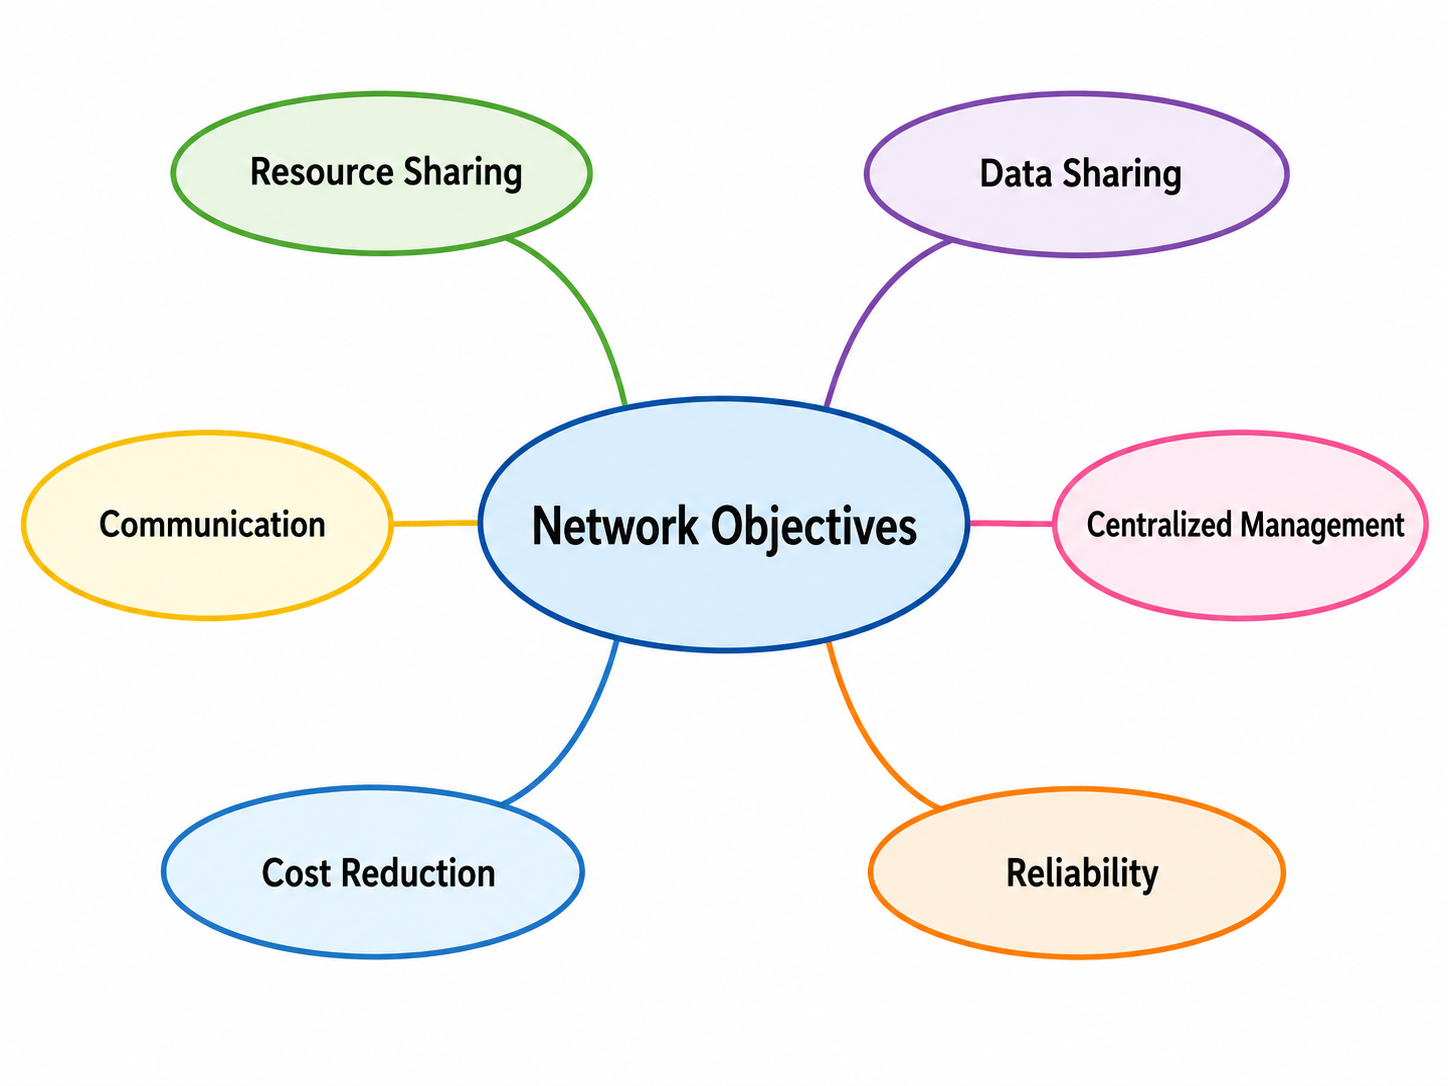
\includegraphics[width=0.92\textwidth]{chapters/Chapter02/images/network_objectives_mindmap.png}
}{
\fbox{
\parbox{0.90\textwidth}{
\centering
\vspace{0.7cm}
Network Objectives\\[8pt]
Resource Sharing \quad Data Sharing \quad Communication\\[6pt]
Centralized Management \quad Cost Reduction \quad Reliability
\vspace{0.7cm}
}}
}
\caption{কম্পিউটার নেটওয়ার্কের উদ্দেশ্য}
\end{figure}

\subsection{Resource Sharing}

\begin{definitionbox}{Resource Sharing}
একটি network-এর একাধিক user বা device একই hardware, software, data বা service ব্যবহার করতে পারাকে resource sharing বলা হয়।
\end{definitionbox}

Resource sharing computer network-এর সবচেয়ে গুরুত্বপূর্ণ উদ্দেশ্যগুলোর একটি। একটি printer network-এ share করলে lab-এর সব computer সেই printer ব্যবহার করতে পারে। একইভাবে file server, database server, internet connection, software license, storage device ইত্যাদিও share করা যায়।

\begin{keypointbox}{Resource sharing-এর উদাহরণ}
\begin{itemize}
\item এক printer অনেক computer ব্যবহার করা।
\item file server থেকে class note download করা।
\item office database একাধিক employee ব্যবহার করা।
\item এক internet connection router দিয়ে অনেক device-এ share করা।
\item cloud storage ব্যবহার করে file access করা।
\end{itemize}
\end{keypointbox}

\subsection{Data Sharing}

\begin{definitionbox}{Data Sharing}
Network-এর মাধ্যমে এক device থেকে অন্য device-এ file, document, image, audio, video বা database information আদান-প্রদান করাকে data sharing বলা হয়।
\end{definitionbox}

Data sharing-এর ফলে একই data অনেক user ব্যবহার করতে পারে। এতে duplicate file কমে, কাজ দ্রুত হয় এবং team collaboration সহজ হয়। তবে data sharing-এর ক্ষেত্রে permission, authentication ও backup গুরুত্বপূর্ণ।

\begin{examplebox}{বাস্তব উদাহরণ}
একটি college office-এ admission database server-এ রাখা হলো। Principal, office assistant এবং accounts section নির্দিষ্ট permission অনুযায়ী database access করতে পারে। এটি data sharing-এর উদাহরণ।
\end{examplebox}

\subsection{Communication}

Computer network-এর মাধ্যমে userরা দ্রুত communication করতে পারে। Email, instant messaging, video conference, file transfer, online meeting, VoIP call—সবই network-based communication।

\begin{keypointbox}{Network communication-এর সুবিধা}
\begin{itemize}
\item দ্রুত message পাঠানো যায়।
\item দূরবর্তী user-এর সাথে real-time communication করা যায়।
\item video conference ও online class করা যায়।
\item file transfer ও collaborative work সহজ হয়।
\item organization-এর internal communication দ্রুত হয়।
\end{itemize}
\end{keypointbox}

\subsection{Centralized Management}

\begin{definitionbox}{Centralized Management}
Network-এর data, user account, security, printer, software update ও access permission একটি central server বা administrator-এর মাধ্যমে পরিচালনা করার ব্যবস্থাকে centralized management বলা হয়।
\end{definitionbox}

Centralized management বড় office, bank, university ও data center-এর জন্য খুব গুরুত্বপূর্ণ। এতে user account control, password policy, file permission, software update, backup এবং security monitoring সহজ হয়।

\begin{examplebox}{সহজ উদাহরণ}
School lab-এর সব computer-এ আলাদা আলাদা software install না করে server বা administrator centralভাবে software update করলে সময় ও খরচ কমে।
\end{examplebox}

\subsection{Cost Reduction}

Network ব্যবহার করলে hardware ও service share করা যায়। এতে প্রতিটি computer-এর জন্য আলাদা printer, storage বা internet connection প্রয়োজন হয় না। ফলে cost কমে।

\begin{keypointbox}{Cost reduction-এর কারণ}
\begin{itemize}
\item এক printer অনেক computer ব্যবহার করতে পারে।
\item এক internet connection অনেক device-এ share করা যায়।
\item central storage ব্যবহারে আলাদা storage cost কমে।
\item software ও maintenance centralভাবে manage করা যায়।
\item office automation-এর ফলে সময় ও শ্রম কম লাগে।
\end{itemize}
\end{keypointbox}

\subsection{Reliability ও Backup}

Network ব্যবহার করলে data server বা cloud storage-এ backup রাখা যায়। কোনো computer নষ্ট হলেও server বা backup থেকে data restore করা সম্ভব। বড় organization-এ data loss কমাতে network backup system গুরুত্বপূর্ণ।

\begin{mistakebox}{Common mistake}
অনেকে ভাবে network শুধু internet ব্যবহারের জন্য তৈরি করা হয়। আসলে network-এর উদ্দেশ্য resource sharing, data sharing, communication, security, backup, centralized management এবং cost reduction—সবই।
\end{mistakebox}

\subsection{কম্পিউটার নেটওয়ার্কের সুবিধা}

\begin{keypointbox}{সুবিধা}
\begin{itemize}
\item data ও resource সহজে share করা যায়।
\item communication দ্রুত হয়।
\item printer, storage, internet connection share করে cost কমানো যায়।
\item central management ও monitoring করা যায়।
\item data backup ও recovery সহজ হয়।
\item team work ও collaboration বৃদ্ধি পায়।
\item দূরবর্তী access ও cloud service ব্যবহার করা যায়।
\end{itemize}
\end{keypointbox}

\subsection{কম্পিউটার নেটওয়ার্কের অসুবিধা}

\begin{keypointbox}{অসুবিধা}
\begin{itemize}
\item network setup ও maintenance cost থাকতে পারে।
\item security risk থাকে; unauthorized access হতে পারে।
\item virus বা malware network-এর মাধ্যমে ছড়াতে পারে।
\item server down হলে অনেক user service পেতে সমস্যা হতে পারে।
\item skilled network administrator দরকার হতে পারে।
\item network congestion হলে speed কমে যেতে পারে।
\item data privacy রক্ষা করা challenging হতে পারে।
\end{itemize}
\end{keypointbox}

\subsection{কম্পিউটার নেটওয়ার্কের প্রকারভেদ}

Computer network বিভিন্ন ভিত্তিতে শ্রেণিবিভাগ করা যায়। HSC ICT-তে সবচেয়ে গুরুত্বপূর্ণ হলো geographical area বা বিস্তৃতির ভিত্তিতে network classification।

\begin{figure}[H]
\centering
\IfFileExists{chapters/Chapter02/images/network_types_by_area.png}{
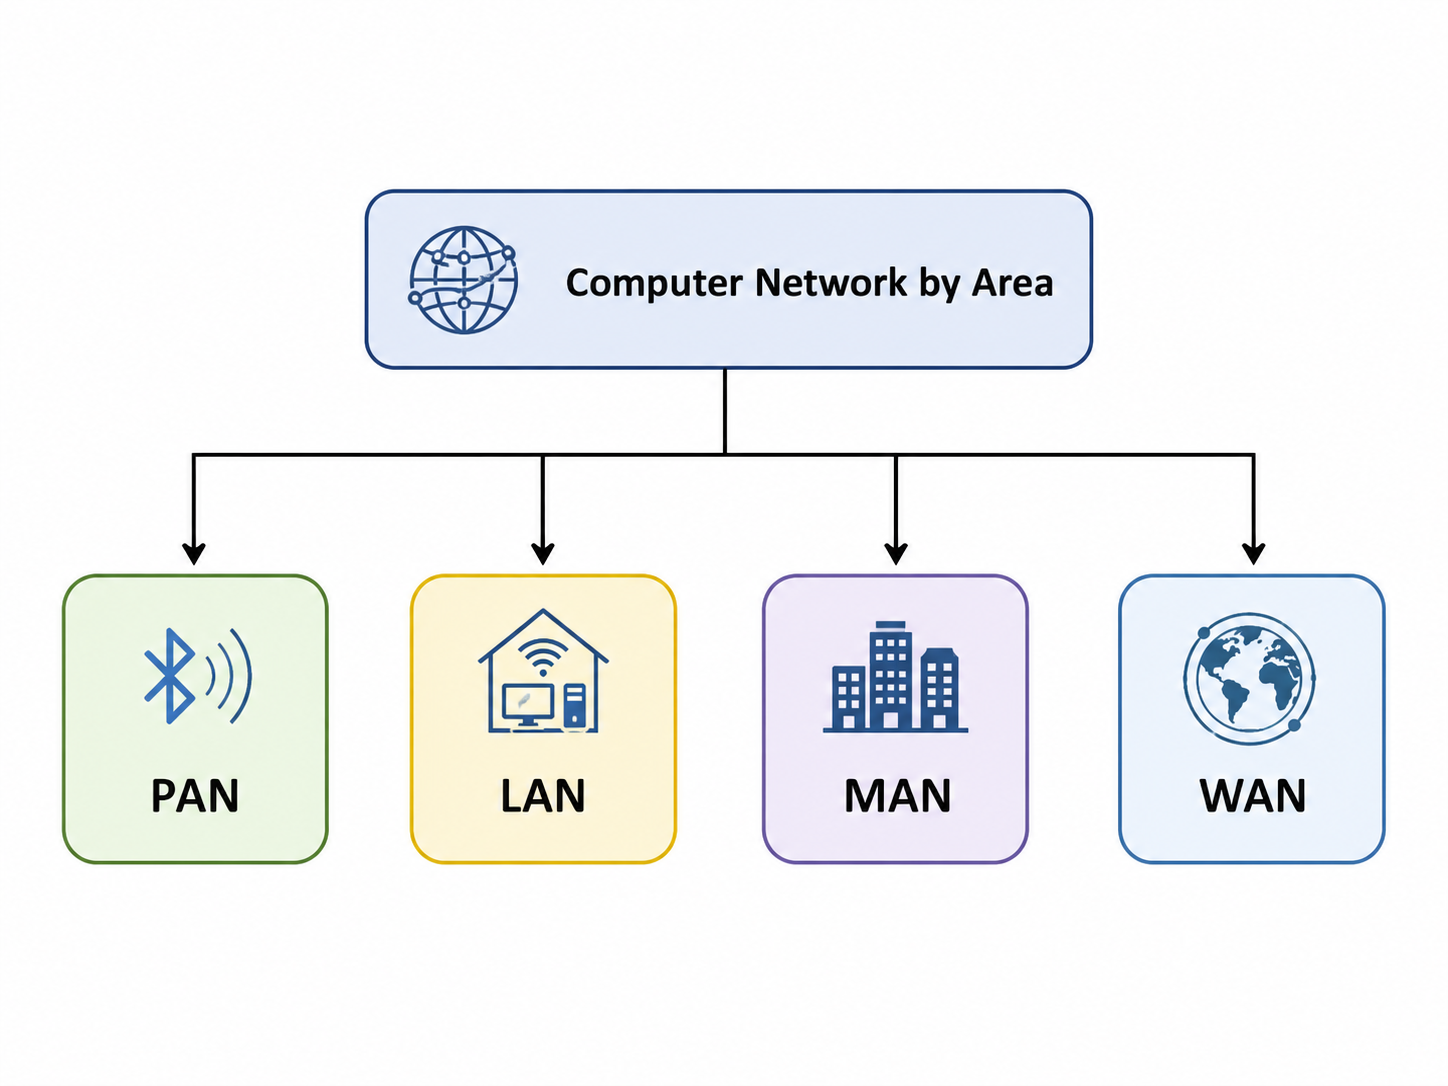
\includegraphics[width=0.92\textwidth]{chapters/Chapter02/images/network_types_by_area.png}
}{
\fbox{
\parbox{0.90\textwidth}{
\centering
\vspace{0.7cm}
Computer Network by Area\\[8pt]
PAN \quad LAN \quad MAN \quad WAN
\vspace{0.7cm}
}}
}
\caption{বিস্তৃতির ভিত্তিতে কম্পিউটার নেটওয়ার্কের প্রকারভেদ}
\end{figure}

\subsection{PAN: Personal Area Network}

\begin{definitionbox}{PAN}
একজন ব্যক্তির নিকটবর্তী personal device-গুলোর মধ্যে স্বল্প দূরত্বে data communication-এর জন্য গঠিত network-কে Personal Area Network বা PAN বলা হয়।
\end{definitionbox}

PAN সাধারণত একজন ব্যক্তির mobile, laptop, smartwatch, wireless earphone, keyboard, mouse, printer ইত্যাদি device-এর মধ্যে তৈরি হয়। Bluetooth, USB cable, infrared বা Wi-Fi Direct ব্যবহার করে PAN তৈরি হতে পারে। PAN-এর coverage সাধারণত খুব ছোট, যেমন কয়েক meter বা personal workspace-এর মধ্যে।

\begin{keypointbox}{PAN-এর বৈশিষ্ট্য}
\begin{itemize}
\item ব্যক্তিগত device-এর মধ্যে communication হয়।
\item coverage area খুব ছোট।
\item সাধারণত low power technology ব্যবহৃত হয়।
\item Bluetooth-based connection PAN-এর পরিচিত উদাহরণ।
\item mobile phone, smartwatch, earphone, keyboard, mouse connect করতে ব্যবহৃত হয়।
\end{itemize}
\end{keypointbox}

\begin{examplebox}{PAN উদাহরণ}
Mobile phone-এর সাথে Bluetooth earphone, smartwatch ও wireless keyboard connect করলে সেটি PAN-এর উদাহরণ।
\end{examplebox}

\subsection{LAN: Local Area Network}

\begin{definitionbox}{LAN}
একটি ছোট geographical area, যেমন room, lab, building, office বা campus-এর মধ্যে computer ও device-গুলোকে সংযুক্ত করে তৈরি network-কে Local Area Network বা LAN বলা হয়।
\end{definitionbox}

LAN সবচেয়ে বেশি ব্যবহৃত network type। School computer lab, office network, home Wi-Fi network, library network ইত্যাদি LAN-এর উদাহরণ। LAN সাধারণত high speed communication দেয় এবং organization নিজেই এটি manage করতে পারে।

\begin{keypointbox}{LAN-এর বৈশিষ্ট্য}
\begin{itemize}
\item ছোট area cover করে।
\item data transfer speed তুলনামূলক বেশি।
\item ownership সাধারণত private বা organization-based।
\item twisted pair cable, switch, router, Wi-Fi access point ব্যবহার হতে পারে।
\item resource sharing ও file sharing-এর জন্য উপযোগী।
\item maintenance তুলনামূলক সহজ।
\end{itemize}
\end{keypointbox}

\begin{examplebox}{LAN উদাহরণ}
College computer lab-এর সব computer switch-এর মাধ্যমে connected থাকলে সেটি LAN।
\end{examplebox}

\subsection{MAN: Metropolitan Area Network}

\begin{definitionbox}{MAN}
একটি city বা metropolitan area-এর মধ্যে একাধিক LAN বা network-কে সংযুক্ত করে তৈরি বৃহত্তর network-কে Metropolitan Area Network বা MAN বলা হয়।
\end{definitionbox}

MAN সাধারণত LAN-এর চেয়ে বড় কিন্তু WAN-এর চেয়ে ছোট। একটি শহরের বিভিন্ন branch office, bank branch, university campus বা cable TV network MAN-এর উদাহরণ হতে পারে।

\begin{keypointbox}{MAN-এর বৈশিষ্ট্য}
\begin{itemize}
\item একটি শহর বা metropolitan area cover করে।
\item একাধিক LAN সংযুক্ত করতে পারে।
\item LAN-এর চেয়ে coverage বেশি।
\item WAN-এর তুলনায় area ছোট।
\item city-wide broadband, cable TV network বা organization branch connection-এ ব্যবহৃত হতে পারে।
\end{itemize}
\end{keypointbox}

\subsection{WAN: Wide Area Network}

\begin{definitionbox}{WAN}
দেশ, মহাদেশ বা বিশ্বব্যাপী বিস্তৃত বড় geographical area জুড়ে computer ও network-গুলোকে সংযুক্ত করে তৈরি network-কে Wide Area Network বা WAN বলা হয়।
\end{definitionbox}

WAN হলো সবচেয়ে বড় network type। Internet হলো WAN-এর সবচেয়ে পরিচিত উদাহরণ। WAN ব্যবহার করে বিভিন্ন শহর, দেশ বা continent-এর network connected থাকে। WAN-এ leased line, optical fiber backbone, satellite link, microwave link, submarine cable ইত্যাদি ব্যবহার হতে পারে।

\begin{keypointbox}{WAN-এর বৈশিষ্ট্য}
\begin{itemize}
\item খুব বড় geographical area cover করে।
\item দেশ-বিদেশের network সংযুক্ত করে।
\item LAN ও MAN-এর তুলনায় বেশি complex।
\item public/private telecommunication infrastructure ব্যবহার করতে পারে।
\item internet WAN-এর সবচেয়ে পরিচিত উদাহরণ।
\item cost ও management complexity বেশি হতে পারে।
\end{itemize}
\end{keypointbox}

\begin{figure}[H]
\centering
\IfFileExists{chapters/Chapter02/images/pan_lan_man_wan_scale.png}{
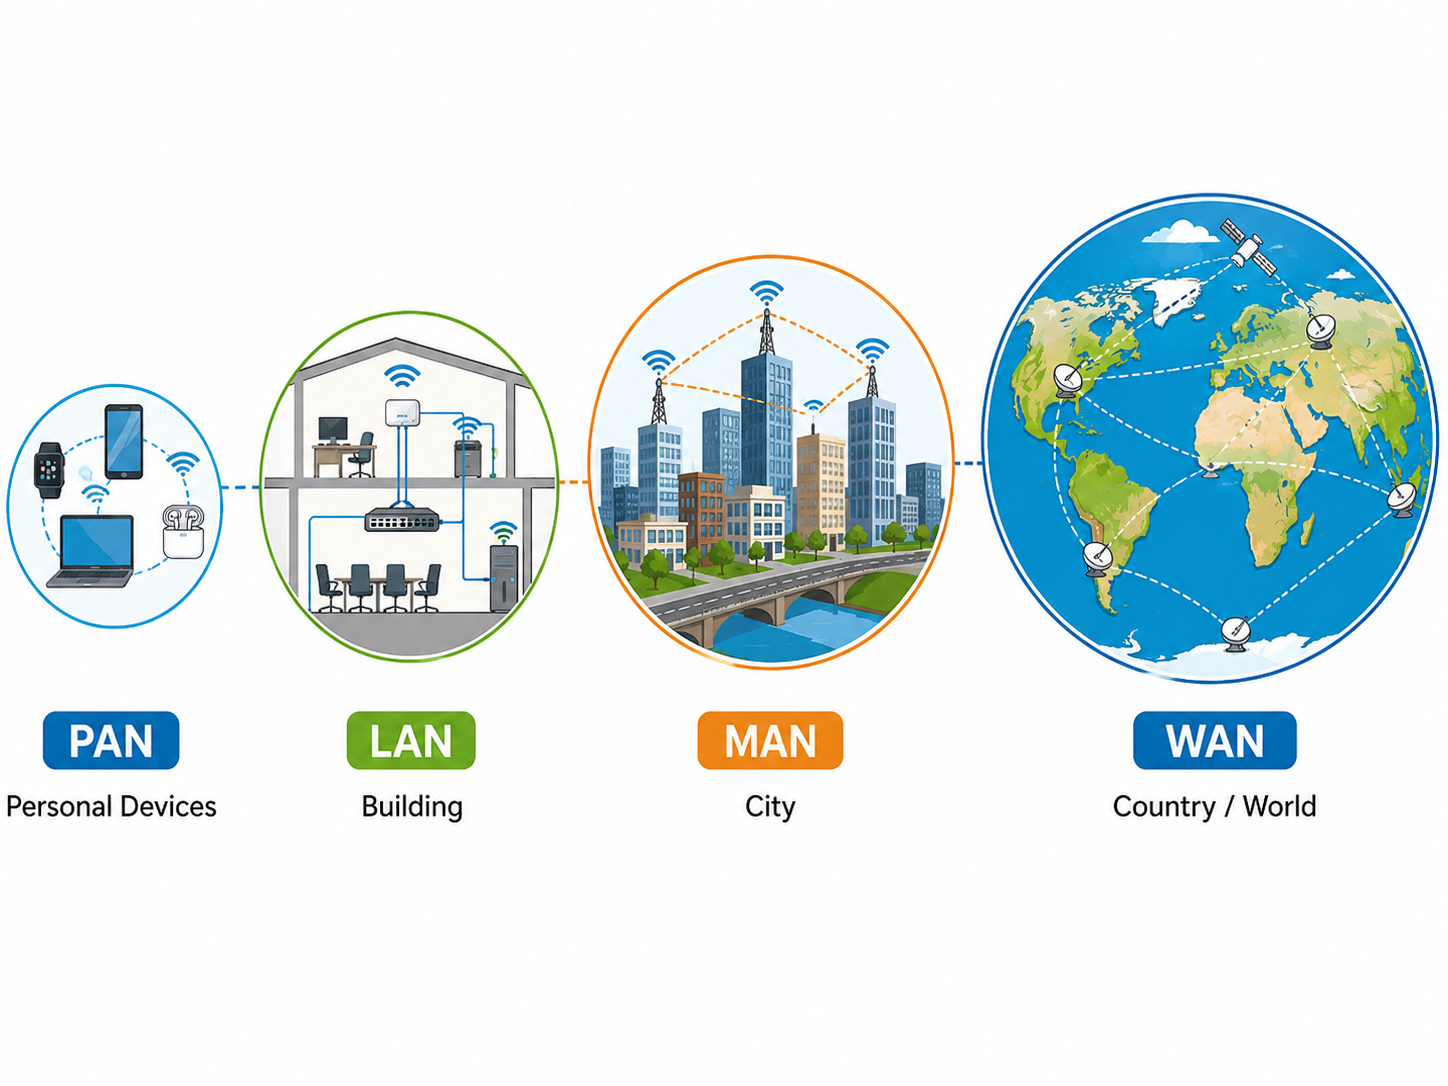
\includegraphics[width=0.92\textwidth]{chapters/Chapter02/images/pan_lan_man_wan_scale.png}
}{
\fbox{
\parbox{0.90\textwidth}{
\centering
\vspace{0.7cm}
PAN: Personal Devices\\[4pt]
LAN: Room / Building\\[4pt]
MAN: City\\[4pt]
WAN: Country / World
\vspace{0.7cm}
}}
}
\caption{PAN, LAN, MAN ও WAN-এর coverage scale}
\end{figure}

\subsection{PAN, LAN, MAN ও WAN-এর পার্থক্য}

\begin{center}
\begin{tabular}{|p{0.14\textwidth}|p{0.20\textwidth}|p{0.26\textwidth}|p{0.28\textwidth}|}
\hline
\textbf{Network} & \textbf{Coverage} & \textbf{ব্যবহার} & \textbf{উদাহরণ} \\
\hline
PAN & ব্যক্তিগত ছোট area & personal device connection & Mobile, smartwatch, Bluetooth earphone \\
\hline
LAN & room, lab, building, campus & local resource sharing & School lab, office network, home Wi-Fi \\
\hline
MAN & city/metropolitan area & city-wide network connection & City broadband, bank branches in a city \\
\hline
WAN & country/worldwide & long-distance communication & Internet, international bank network \\
\hline
\end{tabular}
\end{center}

\begin{boardbox}{বোর্ড ফোকাস}
PAN, LAN, MAN, WAN-এর প্রশ্নে শুধু পূর্ণরূপ লিখলে marks কমতে পারে। Coverage area, ব্যবহার ও উদাহরণ লিখতে হবে।
\end{boardbox}

\subsection{Network Architecture-এর ভিত্তিতে প্রকারভেদ}

Network কে control ও service ব্যবস্থার ভিত্তিতেও ভাগ করা যায়। HSC পর্যায়ে দুটি concept জানা গুরুত্বপূর্ণ:

\begin{itemize}
\item Peer-to-peer Network
\item Client-server Network
\end{itemize}

\subsection{Peer-to-peer Network}

\begin{definitionbox}{Peer-to-peer Network}
যে network-এ প্রতিটি computer প্রায় সমানভাবে resource share করে এবং আলাদা dedicated server থাকে না, তাকে peer-to-peer network বলা হয়।
\end{definitionbox}

Peer-to-peer network ছোট network-এর জন্য উপযোগী। এতে setup সহজ এবং cost কম। তবে security, backup ও centralized control দুর্বল হতে পারে।

\begin{keypointbox}{Peer-to-peer network-এর বৈশিষ্ট্য}
\begin{itemize}
\item dedicated server প্রয়োজন হয় না।
\item প্রতিটি computer resource share করতে পারে।
\item ছোট network-এর জন্য উপযোগী।
\item setup সহজ ও cost কম।
\item security ও management তুলনামূলক দুর্বল।
\end{itemize}
\end{keypointbox}

\subsection{Client-server Network}

\begin{definitionbox}{Client-server Network}
যে network-এ এক বা একাধিক server client computer-গুলোকে file, database, printer, website, authentication বা অন্য service প্রদান করে, তাকে client-server network বলা হয়।
\end{definitionbox}

Client-server network বড় organization, school, bank, hospital, office ও data center-এর জন্য উপযোগী। এখানে server centralভাবে data ও service manage করে। Security, backup, user permission এবং monitoring সহজ হয়।

\begin{keypointbox}{Client-server network-এর বৈশিষ্ট্য}
\begin{itemize}
\item dedicated server থাকে।
\item client server থেকে service নেয়।
\item centralized management করা যায়।
\item security ও backup ভালোভাবে control করা যায়।
\item বড় network-এর জন্য উপযোগী।
\item setup ও maintenance cost বেশি হতে পারে।
\end{itemize}
\end{keypointbox}

\begin{figure}[H]
\centering
\IfFileExists{chapters/Chapter02/images/client_server_vs_peer_to_peer.png}{
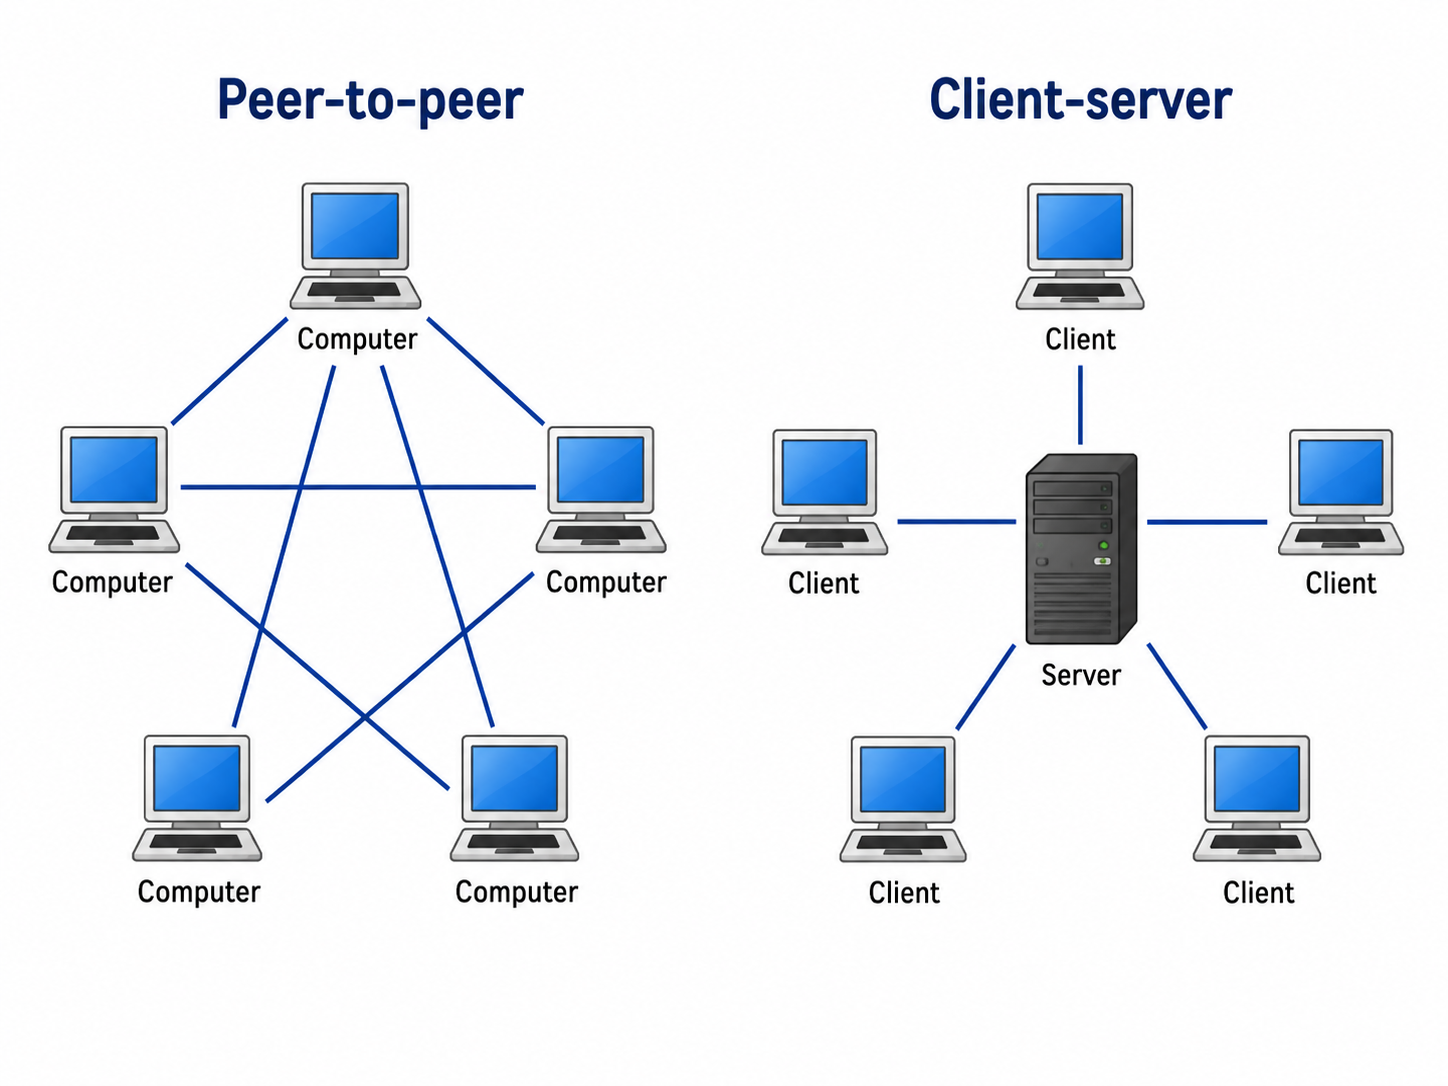
\includegraphics[width=0.92\textwidth]{chapters/Chapter02/images/client_server_vs_peer_to_peer.png}
}{
\fbox{
\parbox{0.90\textwidth}{
\centering
\vspace{0.7cm}
Peer-to-peer: Computer $\longleftrightarrow$ Computer $\longleftrightarrow$ Computer\\[8pt]
Client-server: Client Computers $\longleftrightarrow$ Server
\vspace{0.7cm}
}}
}
\caption{Client-server ও peer-to-peer network}
\end{figure}

\subsection{Client-server ও Peer-to-peer Network-এর পার্থক্য}

\begin{center}
\begin{tabular}{|p{0.24\textwidth}|p{0.30\textwidth}|p{0.30\textwidth}|}
\hline
\textbf{বিষয়} & \textbf{Peer-to-peer} & \textbf{Client-server} \\
\hline
Server & dedicated server নেই & dedicated server থাকে \\
\hline
Control & distributed & centralized \\
\hline
Cost & কম & বেশি \\
\hline
Security & তুলনামূলক কম & ভালোভাবে control করা যায় \\
\hline
উপযোগিতা & ছোট network & বড় organization network \\
\hline
Backup & কঠিন হতে পারে & central backup সহজ \\
\hline
Management & সহজ কিন্তু limited & professional management দরকার \\
\hline
\end{tabular}
\end{center}

\subsection{Internet, Intranet ও Extranet}

\begin{definitionbox}{Internet}
বিশ্বব্যাপী অসংখ্য network-এর সংযোগে গঠিত বৃহত্তম public network-কে Internet বলা হয়।
\end{definitionbox}

\begin{definitionbox}{Intranet}
কোনো organization-এর internal private network, যা সাধারণত organization-এর member বা employee-দের জন্য সীমাবদ্ধ থাকে, তাকে intranet বলা হয়।
\end{definitionbox}

\begin{definitionbox}{Extranet}
কোনো organization-এর private network-এর নির্দিষ্ট অংশ যখন authorized external user, partner, supplier বা customer-এর জন্য সীমিতভাবে উন্মুক্ত করা হয়, তাকে extranet বলা হয়।
\end{definitionbox}

\begin{figure}[H]
\centering
\IfFileExists{chapters/Chapter02/images/internet_intranet_extranet.png}{
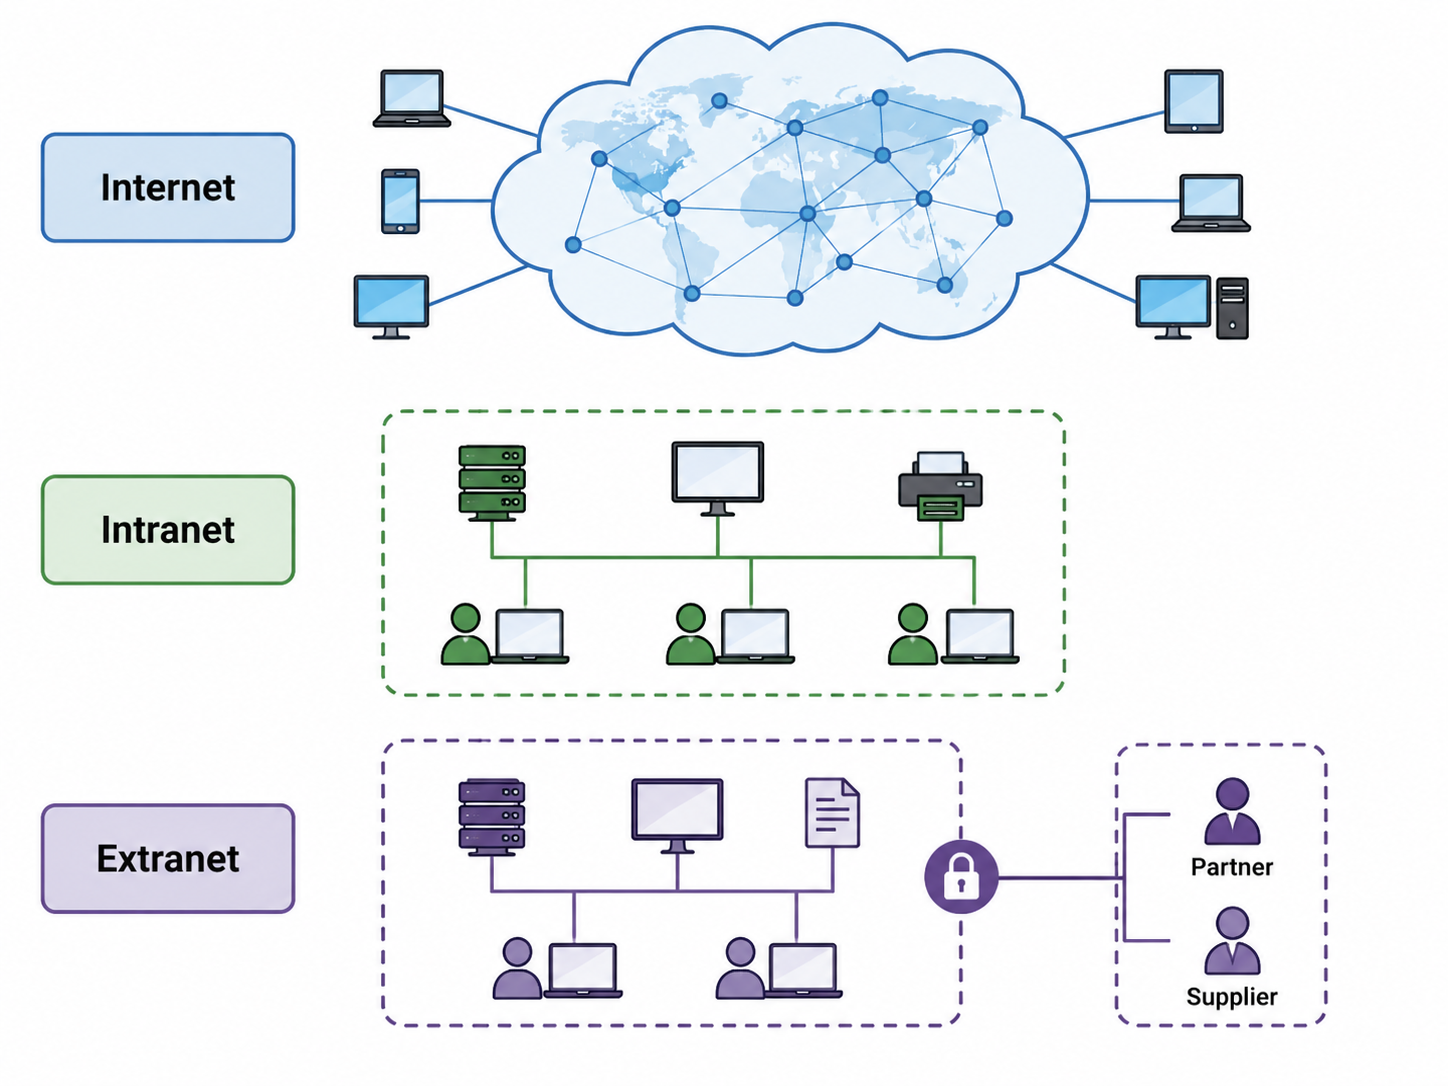
\includegraphics[width=0.92\textwidth]{chapters/Chapter02/images/internet_intranet_extranet.png}
}{
\fbox{
\parbox{0.90\textwidth}{
\centering
\vspace{0.7cm}
Internet: Public Global Network\\[6pt]
Intranet: Private Internal Network\\[6pt]
Extranet: Private Network with Authorized External Access
\vspace{0.7cm}
}}
}
\caption{Internet, Intranet ও Extranet}
\end{figure}

\begin{center}
\begin{tabular}{|p{0.20\textwidth}|p{0.32\textwidth}|p{0.32\textwidth}|}
\hline
\textbf{Network} & \textbf{Access} & \textbf{উদাহরণ} \\
\hline
Internet & public access & Website, email, online service \\
\hline
Intranet & organization internal access & Office internal portal \\
\hline
Extranet & authorized external access & Supplier/customer portal \\
\hline
\end{tabular}
\end{center}

\subsection{বাস্তব scenario অনুযায়ী network নির্বাচন}

\begin{center}
\begin{tabular}{|p{0.32\textwidth}|p{0.20\textwidth}|p{0.32\textwidth}|}
\hline
\textbf{পরিস্থিতি} & \textbf{Network type} & \textbf{কারণ} \\
\hline
Mobile phone ও Bluetooth earphone connection & PAN & personal device, short range \\
\hline
School computer lab & LAN & small area, resource sharing \\
\hline
এক শহরের বিভিন্ন bank branch connection & MAN & city-wide network \\
\hline
International company-এর country-to-country network & WAN & large geographical coverage \\
\hline
Office employee-only portal & Intranet & internal private access \\
\hline
Supplier login portal & Extranet & authorized external access \\
\hline
\end{tabular}
\end{center}

\subsection{Common Mistake Zone}

\begin{mistakebox}{Common mistake ১}
LAN মানে শুধু cable network নয়। Wi-Fi দিয়েও LAN তৈরি হতে পারে, যদি তা local area-এর মধ্যে network তৈরি করে।
\end{mistakebox}

\begin{mistakebox}{Common mistake ২}
Internet ও WAN একই কথা নয়। Internet হলো WAN-এর সবচেয়ে বড় ও পরিচিত উদাহরণ; কিন্তু সব WAN internet নয়।
\end{mistakebox}

\begin{mistakebox}{Common mistake ৩}
PAN ও LAN গুলিয়ে ফেলা যাবে না। PAN ব্যক্তিগত device-এর ছোট network, LAN হলো room/building/campus-এর local network।
\end{mistakebox}

\begin{mistakebox}{Common mistake ৪}
Peer-to-peer network-এ কোনো server concept থাকতে পারে না—এভাবে বলা ঠিক নয়। Dedicated central server থাকে না, কিন্তু প্রতিটি computer নিজ resource share করতে পারে।
\end{mistakebox}

\subsection{Exam-style প্রশ্ন ও উত্তর}

\begin{boardbox}{সংক্ষিপ্ত প্রশ্ন: Computer network কী?}
দুই বা ততোধিক computer, device বা node-কে communication medium ও protocol-এর মাধ্যমে যুক্ত করে data, information, hardware, software ও network resource আদান-প্রদানের ব্যবস্থাকে computer network বলা হয়। যেমন—school lab network, office network, internet।
\end{boardbox}

\begin{boardbox}{সংক্ষিপ্ত প্রশ্ন: Computer network-এর উদ্দেশ্য লেখ।}
Computer network-এর প্রধান উদ্দেশ্য হলো resource sharing, data sharing, দ্রুত communication, centralized management, cost reduction, backup ও reliability নিশ্চিত করা। Network-এর মাধ্যমে printer, file, database, internet connection ও software service share করা যায়।
\end{boardbox}

\begin{boardbox}{সংক্ষিপ্ত প্রশ্ন: LAN কী?}
একটি ছোট geographical area, যেমন room, lab, building, office বা campus-এর মধ্যে computer ও device-গুলোকে সংযুক্ত করে তৈরি network-কে LAN বা Local Area Network বলা হয়। School computer lab, office network ও home Wi-Fi LAN-এর উদাহরণ।
\end{boardbox}

\begin{boardbox}{পার্থক্য: LAN ও WAN}
LAN ছোট geographical area যেমন room, building বা campus-এর মধ্যে ব্যবহৃত হয় এবং সাধারণত high speed local communication দেয়। WAN দেশ, মহাদেশ বা বিশ্বব্যাপী বিস্তৃত network, যা long-distance communication করে। School lab network LAN-এর উদাহরণ, আর Internet WAN-এর উদাহরণ।
\end{boardbox}

\begin{boardbox}{পার্থক্য: Client-server ও Peer-to-peer Network}
Peer-to-peer network-এ dedicated server থাকে না এবং প্রতিটি computer resource share করতে পারে। এটি ছোট network-এর জন্য উপযোগী। Client-server network-এ dedicated server থাকে, client-রা server থেকে service নেয় এবং centralized management করা যায়। এটি বড় organization network-এর জন্য উপযোগী।
\end{boardbox}

\subsection{Brainstorming Critical Question}

\begin{practicebox}
একটি কলেজে নতুন digital system চালু করা হলো। Computer lab-এর ৪০টি computer একই printer ও internet connection ব্যবহার করছে। Principal office ও accounts section একই student database access করছে। College-এর দুইটি branch একই শহরে connected এবং head office অন্য জেলায় অবস্থিত।

\begin{enumerate}
\item ক. Computer network কী?
\item খ. Resource sharing কেন গুরুত্বপূর্ণ?
\item গ. Computer lab-এর network কোন type-এর হতে পারে? ব্যাখ্যা কর।
\item ঘ. একই শহরের branch connection ও অন্য জেলার head office connection-এর ক্ষেত্রে MAN ও WAN-এর ব্যবহার বিশ্লেষণ কর।
\end{enumerate}
\end{practicebox}

\subsection{১ মিনিটে রিভিশন}

\begin{recapbox}
\begin{itemize}
\item Computer network হলো connected device-এর system।
\item Networking হলো network তৈরি ও পরিচালনার process।
\item Network-এর উদ্দেশ্য: resource sharing, data sharing, communication, centralized management, cost reduction।
\item PAN ব্যক্তিগত device-এর ছোট network।
\item LAN room/building/campus-এর local network।
\item MAN city-wide network।
\item WAN country/worldwide network।
\item Internet হলো বিশ্বব্যাপী public network।
\item Intranet হলো organization-এর private internal network।
\item Extranet হলো limited external access সহ private network।
\item Peer-to-peer network ছোট network-এর জন্য সহজ ও কম খরচের।
\item Client-server network বড় organization-এর জন্য secure ও centrally managed।
\end{itemize}
\end{recapbox}

\subsection{অনুশীলন}

\begin{practicebox}
\textbf{MCQ}
\begin{enumerate}
\item দুই বা ততোধিক computer যুক্ত করে data ও resource sharing করার ব্যবস্থাকে কী বলে?\\
ক. Processor \quad খ. Computer network \quad গ. Monitor \quad ঘ. Keyboard

\item PAN-এর পূর্ণরূপ কী?\\
ক. Public Area Network \quad খ. Personal Area Network \quad গ. Private Access Node \quad ঘ. Protocol Area Number

\item School computer lab সাধারণত কোন network-এর উদাহরণ?\\
ক. PAN \quad খ. LAN \quad গ. MAN \quad ঘ. WAN

\item একটি শহরের বিভিন্ন branch office যুক্ত করলে কোন network হতে পারে?\\
ক. PAN \quad খ. LAN \quad গ. MAN \quad ঘ. Cache

\item Internet কোন network-এর সবচেয়ে পরিচিত উদাহরণ?\\
ক. WAN \quad খ. PAN \quad গ. ROM \quad ঘ. CPU

\item Client-server network-এ service প্রদান করে কোনটি?\\
ক. Client \quad খ. Server \quad গ. Mouse \quad ঘ. Keyboard

\item Office-এর internal private network কোনটি?\\
ক. Internet \quad খ. Intranet \quad গ. Extranet \quad ঘ. Bluetooth only

\item Bluetooth earphone ও mobile phone-এর network কোনটি?\\
ক. PAN \quad খ. WAN \quad গ. MAN \quad ঘ. PSTN
\end{enumerate}

\textbf{সংক্ষিপ্ত প্রশ্ন}
\begin{enumerate}
\item Computer network কী?
\item Networking বলতে কী বোঝায়?
\item Computer network-এর পাঁচটি উদ্দেশ্য লেখ।
\item Resource sharing কী? উদাহরণ দাও।
\item PAN, LAN, MAN ও WAN-এর মধ্যে পার্থক্য লেখ।
\item Client-server network কী?
\item Peer-to-peer network কী?
\item Internet, Intranet ও Extranet-এর পার্থক্য লেখ।
\item LAN ও WAN-এর মধ্যে পার্থক্য লেখ।
\item Network-এর সুবিধা ও অসুবিধা লেখ।
\end{enumerate}

\textbf{সৃজনশীল প্রশ্ন}
একটি hospital network তৈরি করা হচ্ছে। Doctor chamber-এর computer-গুলো একই printer ও patient database ব্যবহার করবে। Hospital-এর অন্য branch একই শহরে connected থাকবে। Head office অন্য দেশে অবস্থিত এবং online reporting system থাকবে। Supplier-রা নির্দিষ্ট portal দিয়ে medicine stock update করতে পারবে।

\begin{enumerate}
\item ক. LAN কী?
\item খ. Intranet private network কেন?
\item গ. Doctor chamber-এর computer network কোন type-এর? ব্যাখ্যা কর।
\item ঘ. branch, head office এবং supplier portal-এর ক্ষেত্রে MAN, WAN ও Extranet-এর ব্যবহার বিশ্লেষণ কর।
\end{enumerate}
\end{practicebox}